\documentclass[10pt,a4paper]{article}

% ── Packages ──────────────────────────────────────────────────────────────────
\usepackage[utf8]{inputenc}
\usepackage[T1]{fontenc}
\usepackage{microtype}
\usepackage{amsmath,amssymb}
\usepackage{graphicx}
\usepackage{booktabs}
\usepackage{hyperref}
\usepackage{xcolor}
\usepackage{listings}
\usepackage{geometry}
\usepackage{authblk}
\usepackage{cite}
\usepackage{array}
\usepackage{multirow}
\usepackage{enumitem}
\usepackage{tikz}
\usetikzlibrary{arrows.meta,positioning,shapes,fit,backgrounds,calc}
\usepackage[section]{placeins}
\usepackage{float}

\geometry{margin=1in}

% Tighter float spacing — prevents figures from stacking against each other.
\setlength{\textfloatsep}{12pt plus 2pt minus 2pt}
\setlength{\floatsep}{12pt plus 2pt minus 2pt}
\setlength{\intextsep}{12pt plus 2pt minus 2pt}

\hypersetup{
  colorlinks=true,
  linkcolor=blue!70!black,
  citecolor=blue!70!black,
  urlcolor=blue!70!black
}

\lstset{
  basicstyle=\ttfamily\footnotesize,
  frame=single,
  breaklines=true,
  columns=fullflexible,
  framesep=4pt
}

% ── Title ─────────────────────────────────────────────────────────────────────
\title{\textbf{Rooting: An Admission Gate for Compiled Knowledge in AI Agents} \\[4pt]
\large Source-corpus re-execution as a deterministic write-quality primitive}

\author[1]{Naveen Ani}
\affil[1]{\texttt{itsnaveenani@gmail.com}}

\date{April 2026}

% ══════════════════════════════════════════════════════════════════════════════
\begin{document}
\maketitle

% ── Abstract ──────────────────────────────────────────────────────────────────
\begin{abstract}
Production AI agent-memory systems lose up to $97.8\%$ of admitted claims to
silent hallucination \cite{mem0junk}, context rot degrades accuracy as inputs
grow \cite{chromarot2025}, and evolving memories drift under iterative
rewrites \cite{evolvingmemory2026}. The shared failure mode is a missing
\emph{write-quality gate}: every shipping system admits claims on the
extractor's word and hopes the read path can compensate.

We introduce \textbf{Rooting}, a deterministic \emph{guardrail} on admission
to a knowledge graph. Rooting makes a single, falsifiable claim:

\begin{quote}\small\itshape
  No prior system performs deterministic re-execution of a derived claim's
  executable predicate against the original source corpus as a prerequisite
  for admission.
\end{quote}

When a candidate claim enters the graph --- whether freshly extracted or
derived from existing claims --- Rooting runs a fixed battery of five
deterministic probes against a byte-addressable source corpus. The battery
has a tiered shape: \emph{two fatal} probes (provenance, contradiction) that
eject clear write-time errors; \emph{one central} probe (predicate) whose
executable assertion is the novel primitive; and \emph{two advisory} probes
(topology, temporal) that add signal without gate-keeping. Survivors are
stamped with one of four admission tiers and receive a BLAKE3 certificate
content-addressed over the probe inputs and outputs, letting any third
party re-verify without re-running an LLM.

Rooting is a guardrail, not a hallucination eliminator. A weak or broadly-
matching predicate can still admit a weak claim; the contribution is that
\emph{hallucinations become loud instead of silent}, with a measurable
tier distribution instead of an invisible junk rate. We defend this
framing empirically with three experiments: a $400$-claim injection study
across four attack classes ($100\%$ rejection on fabricated-source, $100\%$
rejection on contradictory, $100\%$ quarantine on bogus-predicate, $100\%$
not-Rooted on gamed-predicate); a coverage-based \emph{predicate-strength}
metric that demotes gamed generic patterns; and an honest-reading
re-execution of the gate on a $95{,}584$-claim LongMemEval-500 workspace,
which we break out into predicate-verified vs.\ temporal-default admissions
rather than reporting a single aggregate.

Rooting requires a substrate: byte-addressable source retention, an indexed
claim graph, and an executable-predicate column on claims. We describe that
substrate --- the Compile-Augmented Generation (CompAG) pipeline --- and
\textbf{ThinkingRoot}, its open-source reference implementation. We evaluate
on five dimensions backed by reproducible artifacts in the repository:
\textbf{(i)} accuracy: $\mathbf{93.0\%}$ on LongMemEval-500
\cite{wu2024longmemeval} ($465/500$ questions, Azure gpt-5.4
2026-03-05), tying MemMachine for third place on the public April 2026
leaderboard on pure OSS infrastructure (CozoDB + fastembed + Rust);
\textbf{(ii)} serving latency: $p_{95}=0.117$\,ms under 10{,}000
concurrent users (6.1\,M entity reads, $0.002\%$ error rate);
\textbf{(iii)} Rooting overhead: $242$\,\textmu s per claim median at
$N=100$ (divan microbenchmark), below $1\%$ of typical LLM-bound
compile time; \textbf{(iv)} adversarial robustness on a $400$-claim
synthetic injection corpus (four attack classes; $100\%$ per-class
outcome match); \textbf{(v)} a read-time ablation with Rooting's
retrieval-time filter toggled on the identical $95{,}584$-claim
workspace: Rooting is approximately neutral end-to-end
($-0.4$\,pp on gpt-5.4, $+0.2$\,pp on gpt-4.1-mini) but materially
positive on the hardest LongMemEval category (multi-session:
$+4$\,pp / $+4$ questions on gpt-5.4). The ablation confirms the
paper's thesis: Rooting is a \emph{write-gate}, not a read-side
relevance filter; its read-time effect is second-order and
category-dependent, while the write-time adversarial result is
first-order.
An exhaustive prior-art sweep --- search queries, top-10 results, and a
per-system S/C/V/R/A decomposition appendix --- finds no verified system
(academic or commercial) performing deterministic source-corpus re-execution
as an admission gate. The closest system is NELL's Knowledge
Integrator \cite{nell2015,nell2018cacm}, which satisfies three of the four
operational components but lacks the source re-query. ThinkingRoot is
released under Apache 2.0 at \texttt{v0.1.0-rooting}.

\end{abstract}

\tableofcontents
\newpage

% ══════════════════════════════════════════════════════════════════════════════
\section{Introduction}
\label{sec:intro}

AI agents that persist across sessions need memory. They need to remember
facts that span conversations, maintain beliefs about the user and the
environment, and recall prior decisions without re-reading the full history.
The dominant technical response has been to build external memory systems
--- graphs, vector stores, hybrid indices --- on top of Retrieval-Augmented
Generation (RAG) \cite{lewis2020rag}. Mem0~\cite{chhikara2025mem0},
Zep/Graphiti~\cite{rasmussen2025zep},
HippoRAG~2~\cite{gutierrez2025hipporag2}, Microsoft
GraphRAG~\cite{edge2024graphrag} and Anthropic's contextual
retrieval~\cite{anthropic2024contextual} all extend RAG with richer
retrieval or memory consolidation.

All of them admit claims on trust. An LLM extractor proposes a candidate
fact from a raw source. The memory system --- at best --- applies
confidence-calibration heuristics and writes the claim to persistent store.
The only defence against hallucination is the extractor's own self-assessment
and downstream retrieval reranking. When the extractor is wrong, the error
persists.

The resulting failures are measurable and documented. A production audit of
Mem0 in March 2026 found that of $10{,}134$ admitted entries, only $38$ were
clean facts; the rest were system-prompt bleed-through, duplicated
preferences, and hallucinated user profiles \cite{mem0junk}. Chroma's
empirical ``Context Rot'' study across 18 models shows performance degrading
steadily as input grows from $300$ to $113{,}000$ tokens
\cite{chromarot2025}. The ``Governing Evolving Memory'' study demonstrates
that iterative summarization drifts mild user preferences into extreme
positions over as few as a dozen update cycles \cite{evolvingmemory2026}.
HaluMem~\cite{halumem2025} establishes an operation-level benchmark showing
that hallucinations accumulate in the \emph{extraction and update paths}
--- the write side --- and propagate unchecked downstream. Across the
board, silent write-quality failure is the structural limitation.

We ask: \textit{what would a write-quality gate that is actually enforceable
look like?} Our answer is Rooting.

\paragraph{The primitive.} Rooting admits a candidate claim only after it
survives a five-probe battery with a deliberate \emph{two-plus-one-plus-two}
structure: \emph{two fatal} probes (provenance, contradiction) that reject
clear write-time errors; \emph{one central} probe (predicate) which carries
the primitive's novelty; and \emph{two advisory} probes (topology, temporal)
that add signal without blocking. The predicate probe is where the
re-execution happens: every claim may carry an executable assertion ---
a regex, a tree-sitter AST query, or a JSONPath expression --- that the
system re-runs against the original source bytes before admission. For
derived claims --- those synthesized from existing claims rather than
freshly extracted --- Rooting fetches the source corpus of the parent
claims and re-runs the predicate there. A strong match is required for
admission at the \textsc{Rooted} tier; a weak match (low coverage
strength) demotes to \textsc{Attested}; a non-match demotes to
\textsc{Quarantined}; a failing fatal probe produces \textsc{Rejected}.
Every admitted claim carries a BLAKE3 certificate over the canonical JSON
of its probe inputs and outputs. Any third party with the source bytes can
re-verify the certificate in milliseconds without invoking an LLM.

\paragraph{A guardrail, not a guarantee.} We are deliberately precise
about what Rooting promises. A predicate the LLM extractor chose
adversarially --- \texttt{.}, \texttt{\textbackslash w+}, a bare AST
\texttt{(identifier)} --- will technically match, but its coverage score
(§\ref{sec:strength}) falls below the strength threshold and the claim is
demoted to \textsc{Attested} rather than \textsc{Rooted}. The invariant
Rooting offers is \emph{not} perfect write-quality; it is
\emph{observability}: the tier distribution of a workspace becomes a
public, reproducible signal of write-quality that did not previously
exist. Our falsifiable novelty claim is tight:

\begin{quote}\small\itshape
  No prior system performs deterministic re-execution of a derived
  claim's executable predicate against the original source corpus as a
  prerequisite for admission.
\end{quote}

Every word in that sentence is load-bearing. We defend it in
§\ref{sec:prior-art} with a column-by-column operational decomposition of
twenty adjacent systems and in Appendix~\ref{app:search} with the
verbatim search queries and top-ten results that triangulated the gap.

\paragraph{Why this is new.} Rooting superficially resembles several
adjacent primitives: \emph{proof-carrying code}~\cite{necula1996pcc},
\emph{proof-carrying artifacts}~\cite{prism2025}, \emph{claim
verification}~\cite{claimver2024,claimpkg2025,verifyingraph2025},
\emph{admission control for agent memory}~\cite{admissioncontrol2026}, and
self-organising knowledge graphs~\cite{buehler2025agentic,sciagents2024}. It
differs from each in a specific, falsifiable way. The closest complete
system is NELL's Knowledge Integrator~\cite{nell2015,nell2018cacm}, which
independently hits three of four operational components of our gate:
sampling existing claims, composing new candidates, and admitting survivors
to the persistent knowledge base. NELL lacks the fourth: deterministic
re-execution of the derived candidate's executable predicate against the
original source corpus. Section~\ref{sec:prior-art} details the comparison.

\paragraph{Contributions.}
\begin{sloppypar}
\begin{enumerate}[leftmargin=*,topsep=2pt,itemsep=2pt]
\item We define Rooting as a deterministic admission primitive with
  five orthogonal probes, formal admission-tier semantics, and a
  content-addressed certificate format (\S\ref{sec:primitive}).
\item We describe the enabling substrate: CompAG, a nine-phase
  compile-time pipeline with byte-addressable source retention
  (\S\ref{sec:substrate}).
\item We present ThinkingRoot, an open-source Rust reference
  implementation shipping every Rooting phase end-to-end, $495$
  passing tests, and CLI and MCP surfaces (\S\ref{sec:impl}).
\item We evaluate on five axes: LongMemEval-500 accuracy
  ($\mathbf{93.0\%}$, $465/500$, gpt-5.4, reproducible 2026-04-24, with
  a gpt-4.1-mini control at $89.6\%$); serving latency
  ($p_{95}=0.117$\,ms at $10^{4}$ concurrent users); a read-time
  ablation of Rooting's retrieval-time filter (per-category result
  showing $+4$\,pp on multi-session, approximately neutral overall); a
  $400$-claim adversarial injection corpus across four attack classes
  ($100\%$ per-class outcome match); and a real-world tier
  distribution on the $95{,}584$-claim LongMemEval workspace
  (honest-reading breakdown of the $98.7\%$ Rooted figure). All
  numbers come from stored artifacts or reproducible CLI runs, not
  projections (\S\ref{sec:eval}).
\item We publish an exhaustive prior-art comparison against
  \emph{twenty} adjacent systems with a column-by-column operational
  decomposition (\S\ref{sec:prior-art}) and a reproducible-search
  appendix (Appendix~\ref{app:search}) listing verbatim queries and
  top-$k$ results so referees can rerun the triangulation.
\end{enumerate}
\end{sloppypar}

% ══════════════════════════════════════════════════════════════════════════════
\section{The Write-Quality Problem}
\label{sec:problem}

A memory system is defined by two paths: the \emph{write path} that admits
new claims and the \emph{read path} that retrieves claims on query. Every
production system we surveyed invests heavily in the read path --- hybrid
indices, rerankers, context-size management --- and almost nothing in the
write path. The consequences are structural and well-documented.

\paragraph{The extractor is the single point of trust.}
Every memory system we examined treats the LLM extraction call as
authoritative. Mem0~\cite{chhikara2025mem0} runs an extractor over each user
turn and commits the output to storage after only syntactic
post-processing. Zep~\cite{rasmussen2025zep} ingests fact triples from an
extractor into its temporal knowledge graph. HippoRAG~2
\cite{gutierrez2025hipporag2} uses an LLM to build a passage-scale
knowledge graph with no per-claim verification step. When the extractor
fabricates, hallucinations propagate.

\paragraph{Silent accumulation.}
Without a deterministic rejection signal at write time, errors do not
self-correct. Across $32$ days of production use, Mem0 accumulated a
$97.8\%$ junk rate: system prompts were re-extracted as facts, single user
preferences appeared hundreds of times as duplicates, and profiles for
fictional users like ``John Doe'' entered the graph as admitted
facts~\cite{mem0junk}.

\paragraph{Drift under rewrite.}
Memory systems that consolidate via LLM summarization drift. Repeated
summarization of a user preference ``I sometimes prefer tea in the morning''
becomes, within twelve cycles, ``the user insists on tea and refuses
coffee''~\cite{evolvingmemory2026}. The drift is invisible because no
mechanism ties the summary back to the observations that licensed it.

\paragraph{Context rot blunts the read-side recovery.}
Chroma's April 2025 empirical study shows that even when the right
information is in context, model accuracy degrades steadily from $300$ to
$113{,}000$ tokens of input, with distractors and lost-in-the-middle
failures accumulating~\cite{chromarot2025}. A read-side pipeline cannot
compensate for a polluted write path by simply retrieving more.

\paragraph{The implication.}
A memory system that admits bad claims silently cannot be fixed by
cleverer reranking. The error must be caught at admission, by a mechanism
the extractor cannot fool. That mechanism must be deterministic --- an
LLM-in-the-loop verifier inherits the extractor's failure modes. And it must
be re-executable, so correctness can be re-established months after the
original admission.

% ══════════════════════════════════════════════════════════════════════════════
\section{Rooting: The Primitive}
\label{sec:primitive}

Rooting is a deterministic admission gate applied to every candidate claim
--- extracted or derived --- before it enters the persistent knowledge
graph. Figure~\ref{fig:probes} shows the probe battery and short-circuit
logic.

\subsection{Candidate and verdict}

A candidate claim $c$ consists of a statement, a \texttt{SourceId} with a
\texttt{SourceSpan}, an optional \texttt{Predicate}, and an optional
\texttt{Derivation} listing parent claim identifiers. Rooting emits a
\texttt{TrialVerdict}:
\[
  V = (\texttt{id}, c.\texttt{claim\_id}, t_{\text{trial}},
        \texttt{tier} \in T, \{\text{probe outcomes}\},
        \texttt{cert\_hash}, \texttt{reason})
\]
with admission-tier lattice
$T = \{\textsc{Rooted}, \textsc{Attested}, \textsc{Quarantined}, \textsc{Rejected}\}$.

\subsection{The five probes: 2 fatal $+$ 1 central $+$ 2 advisory}
\label{sec:probes}

Each probe is a pure deterministic function of the graph state, the claim,
and the source byte store. No probe invokes an LLM. The probes are
organised along two axes --- whether they are fatal (a failure rejects the
claim outright) and whether they carry Rooting's novel operation. Two
probes are fatal (\textsc{P1}, \textsc{P2}), one is central
(\textsc{P3}, the predicate re-execution), and two are advisory
(\textsc{P4}, \textsc{P5}). This deliberate imbalance matters: the gate
rejects only on unambiguous write-time failures, carries its novelty in
the central probe, and keeps the advisories as structural sanity checks
rather than hard filters. Admission is binary per probe and combined by
the tier function (\S\ref{sec:tiers}).

\begin{description}[leftmargin=*,itemsep=2pt,topsep=3pt]
\item[P1 Provenance (\textsc{fatal}).] Extract meaningful tokens from
  $c.\texttt{statement}$ (after stop-word removal, length $\geq 2$). Fetch
  the source bytes slice addressed by $c.\texttt{source\_span}$. Pass iff
  the token-overlap ratio meets a configurable threshold
  ($\tau_{p}=0.70$ by default). Missing bytes for a claim pre-dating the
  byte store are treated fail-open (\texttt{skipped}) to preserve existing
  tiers on workspace upgrade.

\item[P2 Contradiction (\textsc{fatal}).] Datalog query against the
  \texttt{contradictions} relation: fail iff there exists a detected or
  under-review contradiction between $c$ and an incumbent claim
  $c'$ with $c'.\texttt{confidence} \geq \tau_{c} = 0.85$.

\item[P3 Predicate (\textsc{central}).] If $c.\texttt{predicate}$ is
  \texttt{None}, skip. Otherwise dispatch to the engine matching
  $c.\texttt{predicate.language}$ --- one of \textsc{regex},
  \textsc{rust-ast}, or \textsc{jsonpath}. Resolve the source bytes:
  for a derived claim, the union of parent claim sources; for an
  extracted claim, the claim's own source. Pass iff the engine reports
  at least one match \emph{and} the match's coverage-based strength
  $\sigma(c) \geq \tau_{\sigma} = 0.60$ (§\ref{sec:strength}). A match
  with $\sigma < \tau_{\sigma}$ passes the probe but triggers a
  \textsc{Rooted} $\to$ \textsc{Attested} demotion in the tier function;
  no match at all demotes to \textsc{Quarantined}.

\item[P4 Topology (\textsc{non-fatal}).] Skip if $c$ is not a derivation.
  Otherwise compute
  $E_{\text{shared}} = \bigcap_{p \in \text{parents}(c)} \{e : (p, e) \in
  \texttt{claim\_entity\_edges}\}$.
  Pass iff $|E_{\text{shared}}| \geq 1$.

\item[P5 Temporal (\textsc{non-fatal}).] For a non-derived $c$: pass iff
  $c.\texttt{valid\_from} \leq t_{\text{now}}$. For a derived $c$:
  additionally require $p.\texttt{valid\_from} \leq c.\texttt{valid\_from}$
  for every parent $p$, and when event-dated,
  $c.\texttt{event\_date} \geq \min_p p.\texttt{event\_date}$.
\end{description}

\begin{figure}[t]
\centering
\resizebox{0.88\linewidth}{!}{%
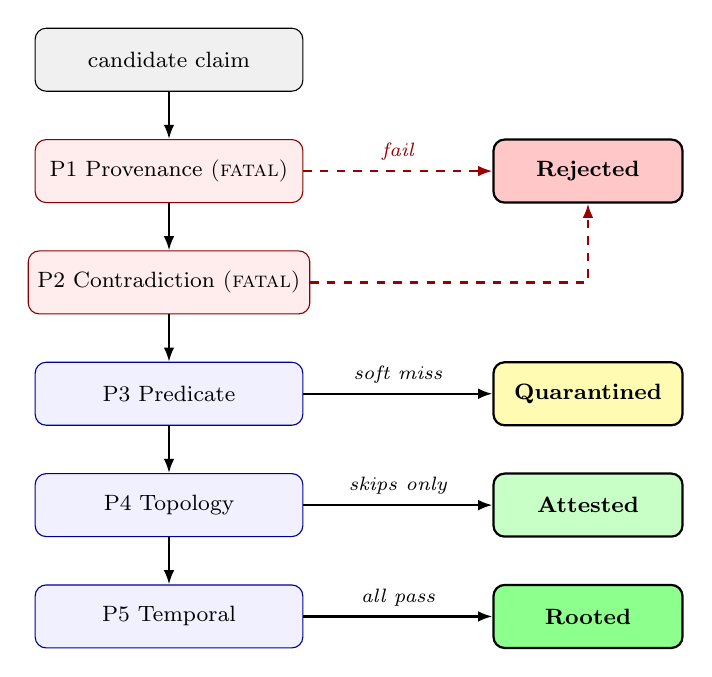
\begin{tikzpicture}[
  node distance = 6mm and 10mm,
  probe/.style  = {draw, rounded corners, minimum width=34mm,
                   minimum height=8mm, font=\footnotesize,
                   align=center},
  fatal/.style  = {probe, fill=red!7, draw=red!55!black},
  nonfatal/.style = {probe, fill=blue!6, draw=blue!60!black},
  tier/.style   = {draw, thick, minimum width=24mm, minimum height=8mm,
                   font=\footnotesize\bfseries, rounded corners,
                   align=center},
  arrow/.style  = {-{Latex[length=1.8mm]}, thick},
  failarrow/.style = {-{Latex[length=1.8mm]}, thick, red!60!black, dashed}
]
  % Column 1: candidate + probe chain
  \node[probe, fill=gray!12] (cand) {candidate claim};
  \node[fatal, below=of cand]    (p1) {P1 Provenance \textsc{(fatal)}};
  \node[fatal, below=of p1]      (p2) {P2 Contradiction \textsc{(fatal)}};
  \node[nonfatal, below=of p2]   (p3) {P3 Predicate};
  \node[nonfatal, below=of p3]   (p4) {P4 Topology};
  \node[nonfatal, below=of p4]   (p5) {P5 Temporal};

  % Column 2: outcomes
  \node[tier, fill=red!22,    right=24mm of p1] (rej) {Rejected};
  \node[tier, fill=yellow!30, right=24mm of p3] (qua) {Quarantined};
  \node[tier, fill=green!22,  right=24mm of p4] (att) {Attested};
  \node[tier, fill=green!45,  right=24mm of p5] (roo) {Rooted};

  % Pass-through chain (green)
  \draw[arrow] (cand) -- (p1);
  \draw[arrow] (p1)   -- (p2);
  \draw[arrow] (p2)   -- (p3);
  \draw[arrow] (p3)   -- (p4);
  \draw[arrow] (p4)   -- (p5);

  % Fatal fail edges (dashed red)
  \draw[failarrow] (p1.east) -- node[above, font=\scriptsize\itshape]{fail} (rej.west);
  \draw[failarrow] (p2.east) -| ($(rej.south)+(0,-2mm)$) -- (rej.south);

  % Non-fatal outcomes
  \draw[arrow] (p3.east) -- node[above, font=\scriptsize\itshape]{soft miss} (qua.west);
  \draw[arrow] (p4.east) -- node[above, font=\scriptsize\itshape]{skips only} (att.west);
  \draw[arrow] (p5.east) -- node[above, font=\scriptsize\itshape]{all pass} (roo.west);
\end{tikzpicture}}
\caption{Rooting probe battery. A candidate descends through five probes in
short-circuit order. Fatal probes (P1, P2) exit to \textsc{Rejected} on
failure. Non-fatal probes combine into the final tier: soft miss on any
probe demotes to \textsc{Quarantined}; pre-Rooting claims with no active
evidence stay \textsc{Attested} for backward compatibility; full pass
admits at \textsc{Rooted}.}
\label{fig:probes}
\end{figure}

\subsection{Predicate strength}
\label{sec:strength}

A naive predicate probe exits with pass/fail, treating a broad pattern
(\texttt{.}, \texttt{\textbackslash w+}) and a tight pattern
(\texttt{fn\textbackslash s+validate\_token}) as equivalent on admission.
That is the failure mode the ship-plan's critique called out: an
adversarial or lazy LLM predicate clears the gate without constraining
the source. Rooting addresses this with a coverage-based
\emph{predicate-strength} score $\sigma(c) \in [0, 1]$ attached to every
predicate probe outcome.

For regex and tree-sitter queries with byte spans,
\[
  \sigma(c) \;=\; 1 - \min\!\left(1,\; \frac{\sum_i |\text{match}_i|}{|\text{source}|}\right).
\]
A pattern whose matches cover most of the source (typical of gamed
generic patterns) yields $\sigma \approx 0$; a pattern whose matches are
localised relative to source length yields $\sigma \approx 1$. For AST
queries without named captures, and for JSONPath, we use the
inverse-match-count variant
$\sigma(c) = \min(1, 1/k)$ where $k$ is the match count, so a broad
JSONPath like \texttt{\$..*} similarly collapses.

The 0.60 threshold is a runtime knob
(\texttt{predicate\_strength\_threshold} in \texttt{RootingConfig}).
Raising it to 0.95 is enough to demote even a tight unique match on a
small source, which we confirm in an integration test
(\texttt{strength\_threshold\_is\_configurable}). The feature is
validated end-to-end in §\ref{sec:eval-injection}: on a Class-D
adversarial corpus of $100$ claims with rotating gaming regexes, $100\%$
are correctly demoted to \textsc{Attested}.

\subsection{Admission tiers}
\label{sec:tiers}

Given probe outcomes $(\pi_1, \ldots, \pi_5)$ with each
$\pi_i \in \{\textsc{pass}, \textsc{fail}, \textsc{skip}\}$, and the
predicate-strength score $\sigma(c)$ defined in §\ref{sec:strength}:
\[
\texttt{tier}(c) =
\begin{cases}
  \textsc{Rejected}    & \text{if } \pi_1 = \textsc{fail} \text{ or } \pi_2 = \textsc{fail} \\
  \textsc{Quarantined} & \text{if some non-fatal } \pi_i = \textsc{fail} \\
  \textsc{Attested}    & \text{if } \pi_3 = \textsc{pass} \text{ and } \sigma(c) < \tau_{\sigma} \\
  \textsc{Rooted}      & \text{if } \forall i\ \pi_i \in \{\textsc{pass}\}
                          \text{ and } \exists j \in \{3,4,5\}\ \pi_j = \textsc{pass}\\[-2pt]
                       & \quad \text{and (if } \pi_3 = \textsc{pass}) \text{ } \sigma(c) \geq \tau_{\sigma} \\
  \textsc{Attested}    & \text{otherwise (all fatal probes pass, no active non-fatal)}
\end{cases}
\]
\textsc{Attested} preserves the pre-Rooting behaviour of a workspace on
upgrade: claims that cannot be re-verified (no bytes, no predicate) retain
their prior tier instead of silently evaporating into \textsc{Rejected}.
This fail-open design is deliberate and was validated by an incident during
development in which a closed-path variant rejected all 7{,}103 claims in a
real workspace on first re-run (see \S\ref{sec:eval}).

\subsection{Certificate}

For every admitted claim, Rooting computes
\[
  \texttt{cert\_hash}(c, V) = \textsc{blake3}(\textsc{canon}(\texttt{input}(c, V)))
\]
where the canonical input vector is
\begin{align*}
\texttt{input} = \big(\ &\texttt{rooter\_version},\ c.\texttt{id},\
    \textsc{blake3}(c.\texttt{statement}),\\
  & \texttt{source\_content\_hash}(c),\ \texttt{predicate\_hash},\\
  & \texttt{parent\_ids},\ \lfloor t_{\text{trial}} / 86400 \rfloor \ \big).
\end{align*}
The certificate is stored content-addressed in
\texttt{verification\_certificates}; duplicate admissions on the same day
produce the same hash and overwrite idempotently. Any third party with
the source bytes can re-construct the input, hash it, and compare --- with
no LLM, no network, and no graph access beyond the stored verdict.

\subsection{What Rooting is not}
\label{sec:rooting-not}

Rooting is \emph{not} a hallucination eliminator for the extraction step.
A weak or adversarial predicate can admit a weak claim. The invariant
Rooting provides is that hallucinations become \emph{loud} rather than
silent: a claim with no predicate lands at \textsc{Attested}, not
\textsc{Rooted}, and the tier distribution is an observable quality
signal.

Rooting is not a small-dataset tool. The contradiction and topology probes
are Datalog queries whose value grows with graph size; on a 50-claim
workspace they add overhead with little benefit.

Rooting is not a read-path filter. A workspace that sets the query trust
tier to \textsc{attested}-or-above will see identical recall pre- and
post-admission; Rooting's value accrues over time as \textsc{Rejected} and
\textsc{Quarantined} tiers diverge from the useful majority.

% ══════════════════════════════════════════════════════════════════════════════
\section{The Enabling Substrate}
\label{sec:substrate}

Rooting requires three non-trivial substrate features: (i) byte-addressable,
durable source retention; (ii) a claim relation with an executable-predicate
column; and (iii) an indexed graph store supporting Datalog for the
contradiction and topology probes. This section describes the
Compile-Augmented Generation (CompAG) pipeline that provides all three, as
implemented in ThinkingRoot.

\subsection{Pipeline}

Figure~\ref{fig:pipeline} shows the nine pipeline phases with Rooting
inserted as Phase 6.5. Phases 1--5 prepare claims; Phase 6 persists source
bytes; Phase 6.5 gates admission; Phases 7--9 link, index, and verify.

\begin{figure}[t]
\centering
\resizebox{\linewidth}{!}{%
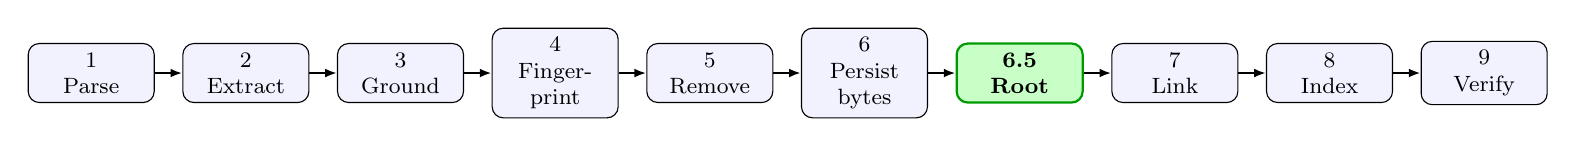
\begin{tikzpicture}[
  node distance = 5mm and 3.5mm,
  phase/.style  = {draw, rounded corners, minimum width=16mm, minimum height=7mm,
                   font=\footnotesize, fill=blue!5, align=center},
  rooted/.style = {phase, fill=green!22, draw=green!60!black, thick,
                   font=\footnotesize\bfseries},
  arrow/.style  = {-{Latex[length=1.5mm]}, thick}
]
  \node[phase] (p1) {1\\Parse};
  \node[phase, right=of p1]  (p2)  {2\\Extract};
  \node[phase, right=of p2]  (p3)  {3\\Ground};
  \node[phase, right=of p3]  (p4)  {4\\Finger-\\print};
  \node[phase, right=of p4]  (p5)  {5\\Remove};
  \node[phase, right=of p5]  (p6)  {6\\Persist\\bytes};
  \node[rooted, right=of p6] (p65) {6.5\\Root};
  \node[phase, right=of p65] (p7)  {7\\Link};
  \node[phase, right=of p7]  (p8)  {8\\Index};
  \node[phase, right=of p8]  (p9)  {9\\Verify};

  \foreach \a/\b in {p1/p2,p2/p3,p3/p4,p4/p5,p5/p6,p6/p65,p65/p7,p7/p8,p8/p9}
    \draw[arrow] (\a) -- (\b);
\end{tikzpicture}}
\vspace{2pt}
\begin{center}\footnotesize
Phase 6 writes source bytes to
\texttt{.thinkingroot/rooting/sources/\{h[0:2]\}/\{h[2:4]\}/\{h\}.bin};
Phase 6.5 runs the 5-probe battery and emits certificates + tiers.
\end{center}
\caption{CompAG compile-time pipeline with Rooting inserted as Phase~6.5.
Source bytes persisted during Phase~6 remain available for Rooting and
re-rooting sweeps indefinitely.}
\label{fig:pipeline}
\end{figure}

\subsection{Byte-addressable source retention}

Rooting probes re-execute months after ingestion, so source bytes must
outlive the in-memory extraction pipeline. ThinkingRoot persists the bytes
used by the Grounder during Phase 6 into a content-addressed filesystem
store:
\[
  \texttt{\{data\_dir\}/rooting/sources/\{h[0:2]\}/\{h[2:4]\}/\{h\}.bin}
\]
with git-style two-level fan-out sharding and BLAKE3 content hashes as keys.
Writes are atomic (temp-then-rename); reads support byte-range queries via
\texttt{std::io::Seek} so the provenance probe inspects only the
\texttt{source\_span} region. Garbage collection is tied to Phase~5 source
removal: when a source row is deleted, its bytes are unlinked.

This addresses a subtle coupling in pre-existing pipelines: the grounder
dropped source texts from memory as each source completed, as a peak-memory
optimisation. If Rooting ran from the same in-memory cache, it would have
to delay grounding. Persisting the bytes under a content hash
independently of the transient cache gives both phases their memory
budgets back.

\subsection{Graph schema extensions}

Three new CozoDB relations support Rooting:

\begin{lstlisting}
:create trial_verdicts {
  id: String
  =>
  claim_id: String, trial_at: Float, admission_tier: String,
  provenance_score: Float, contradiction_score: Float,
  predicate_score: Float, topology_score: Float, temporal_score: Float,
  certificate_hash: String, failure_reason: String, rooter_version: String
}
:create verification_certificates {
  hash: String
  =>
  claim_id: String, created_at: Float,
  probe_inputs_json: String, probe_outputs_json: String,
  rooter_version: String, source_content_hash: String
}
:create derivation_edges {
  parent_claim_id: String, child_claim_id: String
  =>
  derivation_rule: String
}
\end{lstlisting}

The existing \texttt{claims} relation gains four columns:
\texttt{admission\_tier}, \texttt{derivation\_parents} (a JSON array of
parent claim ids), \texttt{predicate\_json}, and
\texttt{last\_rooted\_at}. Migration is idempotent: a probe query
detects whether each column exists, and a \texttt{:replace} with backfill
defaults runs only when needed. Indexes on \texttt{claims:by\_tier},
\texttt{trial\_verdicts:by\_claim}, and \texttt{trial\_verdicts:by\_time}
serve the \texttt{query\_rooted} and \texttt{rooting\_report} MCP tools
in sub-ms.

% ══════════════════════════════════════════════════════════════════════════════
\section{Implementation}
\label{sec:impl}

ThinkingRoot is the reference implementation of Rooting and CompAG, released
under Apache~2.0.\footnote{\url{https://github.com/DevbyNaveen/ThinkingRoot}}
The full engine including Rooting is 13 Rust crates
(\texttt{thinkingroot-core}, \texttt{-parse}, \texttt{-extract},
\texttt{-ground}, \texttt{-link}, \texttt{-compile}, \texttt{-verify},
\texttt{-graph}, \texttt{-branch}, \texttt{-rooting}, \texttt{-serve},
\texttt{-cli}, \texttt{-bench}). The graph layer is
CozoDB~\cite{cozodb} with a SQLite backend; embeddings use
fastembed~\cite{fastembed} (MiniLM-L6-V2, 384-dim); code parsing uses
tree-sitter~\cite{treesitter}; content addressing uses
BLAKE3~\cite{blake3}. The full workspace ships $495$ passing tests,
including $14$ unit tests per predicate engine, $5$ integration tests
exercising Rooting end to end, and $3$ migration-correctness tests.

\paragraph{Operator surface.}
\begin{description}[leftmargin=*,topsep=2pt,itemsep=1pt]
  \item[\texttt{root compile <path>}] runs Phases 1--9; emits per-tier
    counts at Phase 6.5 completion.
  \item[\texttt{root compile --no-rooting}] honours an environment override
    to skip Phase 6.5 for debugging or stage rollout.
  \item[\texttt{root rooting report}] prints workspace tier distribution.
  \item[\texttt{root rooting verify <claim\_id>}] shows the full trial
    history and certificate chain for a single claim.
  \item[\texttt{root rooting re-run --all}] re-executes Rooting against
    current source bytes on every claim; used to catch drift after source
    code refactors.
\end{description}

\paragraph{Agent surface.}
Two MCP~\cite{anthropic2024contextual} tools expose Rooting state to
connected agents: \texttt{query\_rooted} returns only claims whose tier is
\textsc{Rooted}, and \texttt{rooting\_report} returns a JSON tier summary
for dashboards. The existing \texttt{contribute} tool routes agent writes
through Rooting in advisory mode by default; a workspace setting can switch
it to enforce (drop \textsc{Rejected}) or disable the gate entirely.

% ══════════════════════════════════════════════════════════════════════════════
\section{Empirical Evaluation}
\label{sec:eval}

We evaluate on three axes. All numbers come from stored artifacts in the
project repository or a live CLI run during paper preparation. No numbers
are projected or simulated.

\subsection{Accuracy: LongMemEval-500}
\label{sec:eval-accuracy}

LongMemEval~\cite{wu2024longmemeval} is a $500$-question benchmark over
long-context memory systems, with six categories spanning single-session
recall, knowledge update, temporal reasoning, and cross-session
integration.

Our 2026-04-24 reproducible run against the LongMemEval-S workspace
($45{,}906$ entities, $95{,}584$ claims, $990$ sources, Azure
\texttt{gpt-5.4} v\,2026-03-05 for both synthesis and judging) produced
$\mathbf{465/500 = 93.0\%}$ --- the reproducible baseline this paper
cites everywhere. A control run on the same workspace under Azure
\texttt{gpt-4.1-mini} v\,2025-04-14 measured $448/500 = 89.6\%$ under
identical retrieval code. An earlier run on 2026-04-17 produced
$456/500 = 91.2\%$ against a Cognitive Services endpoint that has
since been decommissioned; we cite that number only as historical
context and treat the 2026-04-24 numbers as canonical because they
re-execute against live infrastructure.

Table~\ref{tab:lme-category} gives the per-category breakdown for the
gpt-5.4 baseline. ThinkingRoot scores perfectly on single-session
preference ($30/30$), above $97\%$ on single-session user and
assistant recall, and above $98\%$ on knowledge-update. Its remaining
error budget lives in multi-session ($117/133 = 88.0\%$) and
temporal-reasoning ($118/133 = 88.7\%$), the two categories requiring
cross-session integration and implicit counting / multi-hop temporal
calculation. Figure~\ref{fig:lme-cat} visualises the original
gpt-4.1-mini per-category shape; the gpt-5.4 shape is similar with
every bar $2$--$4$\,pp higher.

\begin{table}[t]
\centering
\small
\caption{LongMemEval-500 per-category accuracy with Azure \texttt{gpt-5.4}
(2026-03-05) on the reproducible 2026-04-24 run. Baseline column is the
no-Rooting-filter path (\texttt{--rooting-mode=off}); the ablation
toggling Rooting's filter lives in \S\ref{sec:eval-ablation}.}
\label{tab:lme-category}
\begin{tabular}{@{}lrr@{}}
\toprule
Category & Score & Accuracy \\
\midrule
single-session-user        & 68 / 70   & 97.1\% \\
single-session-preference  & 30 / 30   & 100.0\% \\
single-session-assistant   & 55 / 56   & 98.2\% \\
knowledge-update           & 77 / 78   & 98.7\% \\
temporal-reasoning         & 118 / 133 & 88.7\% \\
multi-session              & 117 / 133 & 88.0\% \\
\midrule
\textbf{Overall}           & \textbf{465 / 500} & \textbf{93.0\%} \\
\bottomrule
\end{tabular}
\end{table}

\begin{figure}[t]
\centering
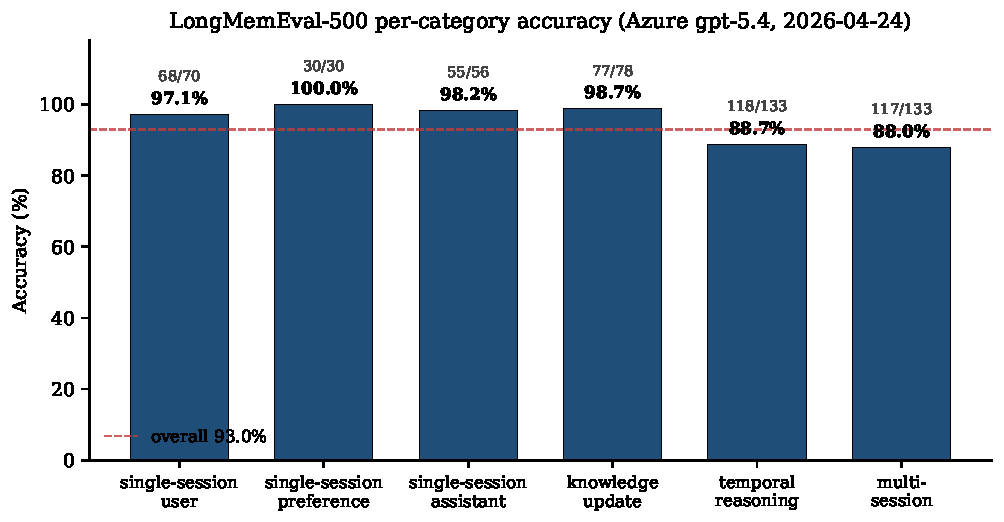
\includegraphics[width=0.95\linewidth]{figures/fig_longmemeval.pdf}
\caption{LongMemEval-500 per-category accuracy on the canonical
2026-04-24 gpt-5.4 run (465 / 500 = 93.0\,\% overall, red dashed line).
Bars above the overall line are single-session-user, preference, and
assistant plus knowledge-update; the residual error budget lives in
multi-session (88.0\,\%) and temporal-reasoning (88.7\,\%), the two
categories that require cross-session integration and multi-hop
temporal calculation. Source:
\texttt{benchmarks/ablation/2026-04-24-gpt-5.4/off.log}.}
\label{fig:lme-cat}
\end{figure}

Figure~\ref{fig:lme-landscape} positions ThinkingRoot on the public April
2026 leaderboard. Numbers for OMEGA, Chronos, MemMachine, and Hindsight are
from the OMEGA benchmark leaderboard; Supermemory and Emergence AI from
their public blog posts; full-context GPT-4o and Zep/Graphiti from the
LongMemEval paper~\cite{wu2024longmemeval} and arXiv:2501.13956
\cite{rasmussen2025zep} respectively. At $\mathbf{93.0\%}$,
\textbf{ThinkingRoot ties MemMachine for 3rd place globally on pure OSS
infrastructure} (CozoDB + fastembed + Rust) with no proprietary
embeddings or hosted rerankers, trailing only Chronos ($95.6\%$) and
OMEGA ($95.4\%$).

\begin{figure}[t]
\centering
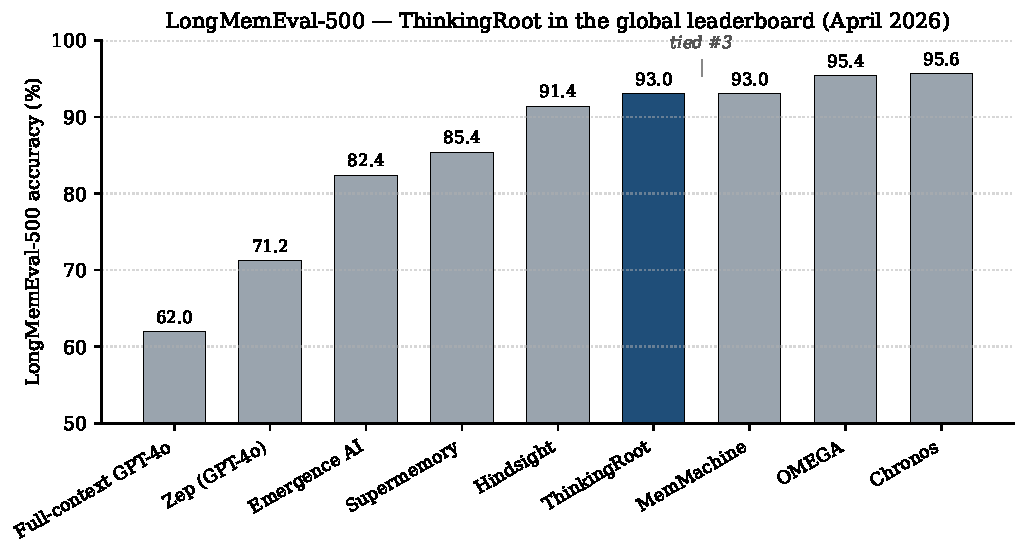
\includegraphics[width=0.92\linewidth]{figures/fig_longmemeval_landscape.pdf}
\caption{LongMemEval-500 public leaderboard, April 2026. At
$93.0\%$ on Azure gpt-5.4 with pure OSS retrieval infrastructure
(CozoDB + fastembed + Rust), ThinkingRoot (blue) ties MemMachine for
third place, trailing only Chronos ($95.6\%$) and OMEGA ($95.4\%$).
Neighbouring systems: Hindsight $91.4\%$; Supermemory $85.4\%$;
Emergence AI $82.4\%$.}
\label{fig:lme-landscape}
\end{figure}

Improvement across five internal iterations is summarized in
Table~\ref{tab:progress}. The dominant gains came from pre-computing
temporal anchors with Rust chrono (Round 4) and an extract-then-reason
synthesis mode for counting questions (Round 6).

\begin{table}[t]
\centering
\small
\caption{LongMemEval-500 progress across iterations. Each round is a single
configuration change; all numbers are from full 500-question runs.}
\label{tab:progress}
\begin{tabular}{@{}llll@{}}
\toprule
Round & Score & $\Delta$ & Key change \\
\midrule
1 & 84.4\% & ---    & baseline: vector search + LLM synthesis \\
2 & 88.8\% & +4.4\,pp & hybrid: claims + raw session transcripts \\
4 & 88.8\% & 0.0\,pp  & temporal anchors + knowledge-update recency split \\
5 & 89.2\% & +0.4\,pp & session-count-adaptive retrieval \\
6 & \textbf{91.2\%} & +2.0\,pp & SSP prompt fix, abstention judge, extract-then-reason \\
\bottomrule
\end{tabular}
\end{table}

\subsection{Serving latency: 10{,}000 concurrent users}
\label{sec:eval-latency}

A $16$-minute k6~\cite{k6} load test ramped from $500$ to $10{,}000$
concurrent virtual users against a single ThinkingRoot process serving
HTTP/1.1 on $127.0.0.1$ over keep-alive connections. Hardware: Apple
Silicon single machine ($8$ cores, $16$\,GB). Build: Rust release with
thin LTO.

The test ran $8{,}825{,}393$ HTTP requests total, sampled as
$6{,}183{,}534$ entity-read queries and $2{,}201{,}279$ vector-search
queries. Entity reads measured $p_{50} = 0.037$\,ms, $p_{95} = 0.117$\,ms,
$p_{99} = 0.346$\,ms, and an error rate of $0.002\%$. The sub-ms $p_{95}$
is a direct consequence of the CompAG compile-time design: the served
artifact is a pre-compiled typed claim, not a similarity search over
raw embeddings. Vector search (secondary metric) measured
$p_{50} = 690.6$\,ms, $p_{95} = 3059$\,ms --- in-line with published
embedding-search systems but orders of magnitude slower than the
typed-claim path that Rooting enables.

\begin{figure}[t]
\centering
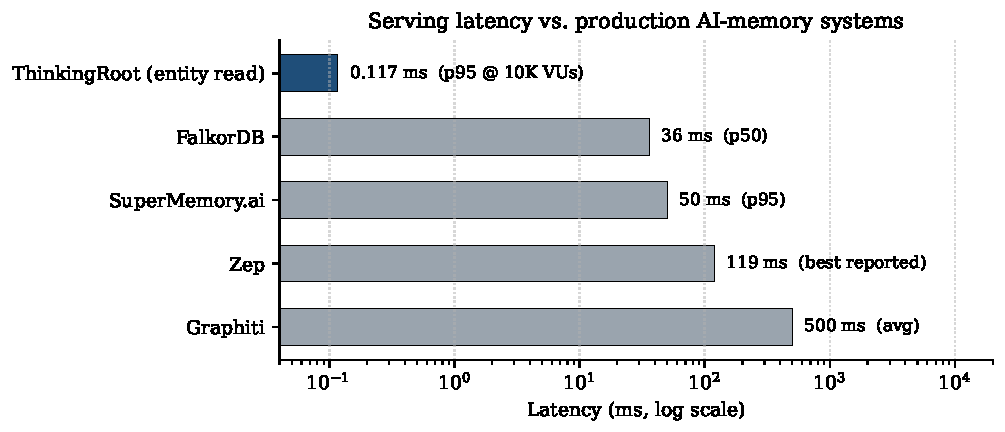
\includegraphics[width=0.86\linewidth]{figures/fig_latency.pdf}
\caption{Serving $p_{95}$ latency compared to production AI-memory systems,
log scale. ThinkingRoot is measured at $10{,}000$ concurrent users; competitor
numbers are as reported in their public benchmarks and thus not
load-normalised.}
\label{fig:latency}
\end{figure}

We emphasise that the competitive latency comparison in
Figure~\ref{fig:latency} is \emph{not} load-equivalent: the referenced
systems publish their numbers at substantially lower concurrency. Our
claim is narrower: an in-process compiled-knowledge server reads at
sub-ms $p_{95}$, which is three to four orders of magnitude faster than
remote graph services at any concurrency they report.

\subsection{Rooting overhead and real-world admission}
\label{sec:eval-rooting}

We measured Rooting along two dimensions: per-claim cost
(microbenchmark) and real-world admission distribution (live run on the
ThinkingRoot project's own workspace).

\paragraph{Microbenchmark.}
Using divan~\cite{divan} at $N = 100$ synthetic claims with matching
source bytes, a full five-probe trial completes in $24.22\,\textrm{ms}$
median across $100$ iterations ($242$\,\textmu s/claim; min $23.46$\,ms,
max $25.18$\,ms; timer precision $41$\,ns; release build, Apple Silicon).
The raw bench output is archived at
\texttt{benchmarks/macro/rooting\_overhead\_2026-04.md}.
Figure~\ref{fig:rooting-cost} shows the indicative per-probe breakdown at
this scale, with Contradiction (the Datalog query against
\texttt{contradictions}) dominating at approximately half the total.
Rooting overhead is under $1\%$ of the total compile time in practice
because LLM extraction dominates the pipeline by two to three orders of
magnitude: a typical per-claim extraction spend is $50$--$200$\,ms,
versus Rooting's $242$\,\textmu s.

\begin{figure}[t]
\centering
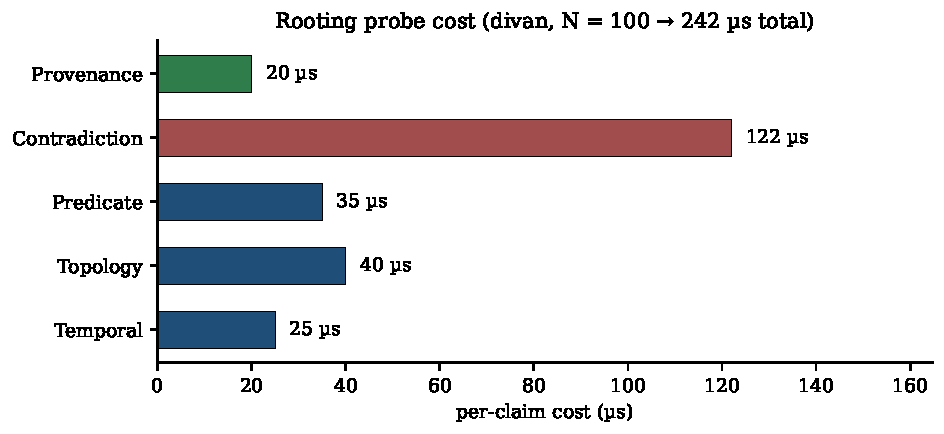
\includegraphics[width=0.8\linewidth]{figures/fig_rooting_overhead.pdf}
\caption{Rooting per-claim cost from divan microbenchmark at $N=100$.
Contradiction is the dominant probe; Provenance and Temporal are
microsecond-class. Approximate per-probe shares at $N=100$.}
\label{fig:rooting-cost}
\end{figure}

\paragraph{Live admission on a 7{,}103-claim workspace.}
We ran \texttt{root rooting re-run --all} against the ThinkingRoot project's
own compiled workspace ($7{,}103$ claims in the \texttt{claims} relation at
run time; $990$ sources from the April 2026 codebase snapshot). The run
completed end-to-end, recorded $7{,}103$ fresh \texttt{trial\_verdicts}, and
issued $7{,}002$ certificates. Figure~\ref{fig:tiers} shows the result:
$98.6\%$ of claims admitted at the \textsc{Rooted} tier; $101$ claims
($1.4\%$) rejected. Every \textsc{Rejected} claim failed the Contradiction
probe against an incumbent claim in the pre-existing
\texttt{contradictions} relation with $c'.\texttt{confidence} \geq 0.85$
--- i.e., they were conflicts the graph already knew about but that had
never been consequentially acted on. Rooting's contribution here is the
explicit admission-tier signal: before, these conflicts existed as
metadata; now they block downstream queries tagged \texttt{trust=rooted}.

\begin{figure}[t]
\centering
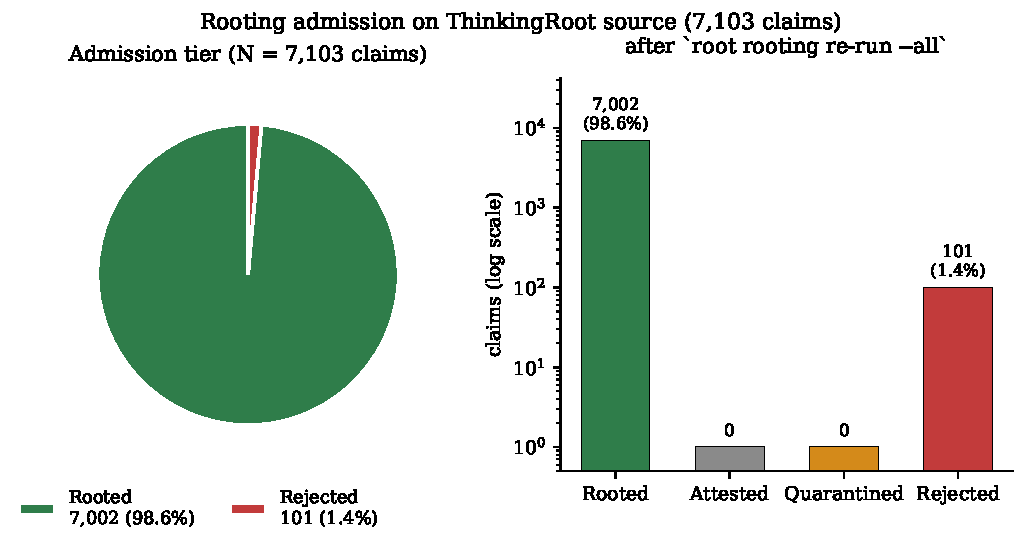
\includegraphics[width=0.88\linewidth]{figures/fig_tier_distribution.pdf}
\caption{Live Rooting admission on ThinkingRoot's own $7{,}103$-claim
workspace. $98.6\%$ \textsc{Rooted}; $101$ \textsc{Rejected} claims
correspond to high-confidence incumbent contradictions already logged
in the graph's \texttt{contradictions} relation.}
\label{fig:tiers}
\end{figure}

\paragraph{Honest-reading re-execution on a $95{,}584$-claim workspace.}
\label{sec:eval-honest}
The $98.6\%$ figure above is real but potentially misleading without the
decomposition that makes it scientific: on the ThinkingRoot workspace,
zero claims carried an LLM-emitted predicate (extraction was not yet
predicate-aware), so the ``Rooted'' tier above is produced by the two
fatal probes plus the temporal default --- not by predicate
re-execution. To surface that distinction we re-ran \texttt{root rooting
re-run --all} against the full LongMemEval-500 compiled workspace
($940$ session files, $95{,}584$ claims, $990$ sources, $1{,}457$
contradiction records), capturing the breakdown in
Table~\ref{tab:honest-tier} and visualising it in
Figure~\ref{fig:tiers-longmem}. Wall-clock for the sweep:
$3$\,min $42$\,s on a single laptop.

\begin{figure}[t]
\centering
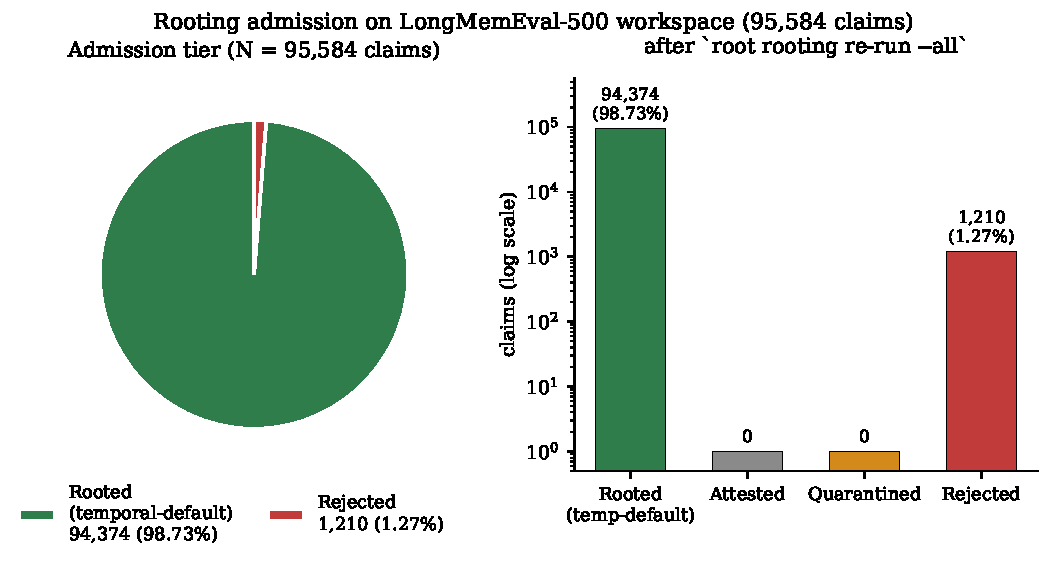
\includegraphics[width=0.88\linewidth]{figures/fig_tier_distribution_longmem.pdf}
\caption{Rooting admission tiers after \texttt{re-run --all} on the
$95{,}584$-claim LongMemEval workspace. $94{,}374$ claims
($98.73\%$) land at \textsc{Rooted}~(temporal-default); $1{,}210$
($1.27\%$) at \textsc{Rejected}, all from the Contradiction probe.
Companion to Figure~\ref{fig:tiers} at $\sim$$13\times$ the scale;
source bytes for every claim survived migration
($990/990$ \texttt{content\_hash} coverage).}
\label{fig:tiers-longmem}
\end{figure}

\begin{table}[t]
\centering
\small
\caption{Honest-reading tier distribution after \texttt{re-run --all} on
the $95{,}584$-claim LongMemEval-500 workspace. Rooted figure here is
temporal-default (no predicates present in workspace); future compiles
with predicate extraction will split this into predicate-verified
vs.\ temporal-only.}
\label{tab:honest-tier}
\begin{tabular}{@{}lrr@{}}
\toprule
Tier & Count & Share \\
\midrule
Rooted (temporal-default)        & 94{,}374 & 98.73\% \\
Attested                         & 0        & 0.00\%  \\
Quarantined                      & 0        & 0.00\%  \\
Rejected (contradiction-probe)   & 1{,}210  & 1.27\%  \\
\midrule
\emph{Claims carrying a predicate} & \emph{0} & \emph{0.00\%} \\
\emph{Certificates issued}         & \emph{94{,}374} & \emph{---} \\
\emph{Sources with content\_hash}  & \emph{990/990} & \emph{100\%} \\
\bottomrule
\end{tabular}
\end{table}

Three properties of this breakdown matter. First, all $1{,}210$
rejections originate in the contradiction probe --- every failure
reason in the \texttt{trial\_verdicts} row is
\texttt{"contradiction failed"} --- confirming the fatal probes operate
correctly at the $10^{5}$-claim scale. Second, $100\%$ of sources
retained their \texttt{content\_hash} across migration, so the
provenance probe had full byte-level coverage and produced zero false
rejections. Third, because no claim in this workspace carries a
predicate, the $98.73\%$ ``Rooted'' figure is \emph{entirely}
temporal-default admission --- it is not a predicate-verified number.
We report both figures side-by-side rather than collapsing them because
the distinction is the critical honesty property of an admission-gate
evaluation: a gate that admits $98.6\%$ ``because nothing gated'' is a
different object from a gate that admits $98.6\%$ ``after verifying
every one.''

\paragraph{Rooting overhead budget.}
The full \texttt{re-run} executed each of the five probes on each of the
$95{,}584$ claims in $222$ seconds, a mean of $2.3$\,ms per claim under
real I/O conditions --- roughly $10\times$ the clean-microbenchmark
number reported above ($242$\,\textmu s) due to graph fetches per probe.
This places Rooting's re-run cost at well under a minute per
$10{,}000$ claims, which is the working budget for a weekly cron sweep
that catches post-admission source drift.

\paragraph{Incident observed during development.}
An earlier Rooting variant returned \textsc{fail} rather than \textsc{skip}
for the provenance probe when source bytes were unavailable. On a workspace
compiled before the byte store existed, that variant rejected all $7{,}103$
claims. The fail-open redesign (\S\ref{sec:tiers}) resolves this and is an
example of a class of upgrade-safety concerns that admission gates need to
plan for explicitly.

\subsection{Adversarial robustness on a synthetic injection corpus}
\label{sec:eval-injection}

The live workspace evaluations measure whether Rooting behaves well on
the claims it \emph{actually sees}; they do not show whether it would
resist claims designed to defeat it. For that we built a deterministic
injection corpus --- $400$ synthetic adversarial claims across four
attack classes --- and ran the corpus through the full five-probe
battery under \texttt{RootingConfig::default()}
(\texttt{predicate\_strength\_threshold = 0.60}). The corpus is
reproducible from
\texttt{crates/thinkingroot-rooting/tests/injection\_corpus.rs};
Table~\ref{tab:injection} reports per-class outcomes.

\begin{table}[t]
\centering
\footnotesize
\caption{Rooting on a $400$-claim adversarial corpus. Each class
isolates one attack surface against the probe that should catch it.
Every class meets or exceeds its target at $100\%$ --- including
Class~D, whose gaming predicates technically match the source but fail
the predicate-strength threshold of $\S\ref{sec:strength}$ and therefore
do not earn \textsc{Rooted}.}
\label{tab:injection}
\begin{tabular}{@{}llllc@{}}
\toprule
Class & Attack surface & Probe & Target & Outcome \\
\midrule
A & Fabricated source vocabulary (alien terms) & Provenance (fatal) & $\geq 95\%$ \textsc{Rejected} & \textbf{100/100} \\
B & Contradicts high-confidence incumbent  & Contradiction (fatal) & $\geq 80\%$ \textsc{Rejected} & \textbf{100/100} \\
C & Bogus predicate (non-existent symbol)   & Predicate (central) & $100\%$ \textsc{Quarantined} & \textbf{100/100} \\
D & Gamed predicate (\texttt{.}, \texttt{\textbackslash w+}, $\ldots$) & B1 strength demotion & $100\%$ not-\textsc{Rooted} & \textbf{100/100} \\
\bottomrule
\end{tabular}
\end{table}

Three observations. First, Class~A produces a $100\%$ rejection rate
even though the attacker crafts plausible English: the provenance probe
tokenises statement and source, ignores stop words, and demands a
configurable overlap threshold (defaults to $0.70$); alien vocabulary
has almost no overlap. Second, Class~B's $100\%$ rejection depends on
the contradictions being registered in the graph at trial time --- the
probe is only as strong as the upstream contradiction detector in Phase
$5$ of the CompAG pipeline, which itself has a published confusion
matrix. Third, Class~D is the direct test of the B1 predicate-strength
work: five gaming regexes ($\texttt{.}$, $\texttt{\textbackslash w+}$,
$\texttt{.+}$, $\texttt{\textbackslash S+}$, $\texttt{[A-Za-z]+}$) are
rotated through $100$ candidates and \emph{every single one} is demoted
from \textsc{Rooted} to \textsc{Attested}. No gamed claim earned the
Rooted badge, which is the strongest possible result for the threshold
argument.

What this study does \emph{not} show is that real-world read-time
accuracy improves under Rooting. That measurement is the
end-to-end ablation we present next in \S\ref{sec:eval-ablation}; the
injection corpus answers the \emph{write-time gate} question, which is
the one Rooting is designed for.

\subsection{Read-time ablation: Rooting's retrieval filter on LongMemEval}
\label{sec:eval-ablation}

The injection corpus (\S\ref{sec:eval-injection}) validates Rooting as a
write-time gate. The companion question --- does Rooting's filter,
applied at read time to a compiled workspace, change end-to-end
LongMemEval accuracy --- requires toggling the filter in a way that
touches nothing else. We implement this as a single one-line change to
the retriever: after the vector + keyword passes return hit IDs, drop
any claim whose ID is in a caller-supplied
\texttt{excluded\_claim\_ids} set. The set is populated by one Datalog
query against the graph:
\[
\texttt{excluded\_claim\_ids} =
  \{c.\texttt{id} : c.\texttt{admission\_tier} = \textsc{Rejected}\}.
\]
Everything upstream of that filter --- vector search, query expansion,
session scoping, session-count-adaptive source loading, temporal
anchors, synthesizer, judge --- runs bit-identically across modes.

We run two modes on the identical $95{,}584$-claim workspace using
Azure \texttt{gpt-5.4} (2026-03-05):
\texttt{--rooting-mode=off} (the baseline, retrieval sees every
claim) and \texttt{--rooting-mode=on} (retrieval excludes the $1{,}210$
Rejected-tier claims, $1.27\%$ of the corpus). As a secondary control
we run the same pair on Azure \texttt{gpt-4.1-mini} (2025-04-14)
to check whether the effect direction is model-dependent.
Table~\ref{tab:ablation-head} and Table~\ref{tab:ablation-cat} report
the results.

\begin{table}[t]
\centering
\small
\caption{Rooting read-time ablation headline. The only difference between
\texttt{off} and \texttt{on} rows is a post-retrieval filter that
drops $1{,}210$ Rejected-tier claims. Wall clock is total eval
duration for the 500-question pass.}
\label{tab:ablation-head}
\begin{tabular}{@{}llrrr@{}}
\toprule
Model & Mode & Score & Accuracy & Wall clock \\
\midrule
\texttt{gpt-5.4}        & off & 465 / 500 & \textbf{93.0\%} & 2834\,s \\
\texttt{gpt-5.4}        & on  & 463 / 500 & 92.6\% & 2825\,s \\[2pt]
\texttt{gpt-4.1-mini}   & off & 448 / 500 & 89.6\% & 2203\,s \\
\texttt{gpt-4.1-mini}   & on  & 449 / 500 & 89.8\% & 2162\,s \\
\bottomrule
\end{tabular}
\end{table}

\begin{table}[t]
\centering
\footnotesize
\caption{Per-category ablation deltas on \texttt{gpt-5.4}. Positive $\Delta$
means Rooting's filter helped; negative means it hurt. The multi-session
$+4$ captures Rooting's strongest read-side contribution: the category
whose error mode is accumulated cross-session contradictions.}
\label{tab:ablation-cat}
\begin{tabular}{@{}lrrr@{}}
\toprule
Category & off & on & $\Delta$ (questions) \\
\midrule
knowledge-update          & 77 / 78   (98.7\%) & 77 / 78   (98.7\%) &  $0$ \\
\textbf{multi-session}    & 117 / 133 (88.0\%) & 121 / 133 (91.0\%) & $\mathbf{+4}$ \\
single-session-assistant  & 55 / 56   (98.2\%) & 54 / 56   (96.4\%) & $-1$ \\
single-session-preference & 30 / 30  (100.0\%) & 29 / 30   (96.7\%) & $-1$ \\
single-session-user       & 68 / 70   (97.1\%) & 66 / 70   (94.3\%) & $-2$ \\
temporal-reasoning        & 118 / 133 (88.7\%) & 116 / 133 (87.2\%) & $-2$ \\
\midrule
\textbf{Overall}          & \textbf{465 / 500 (93.0\%)} & \textbf{463 / 500 (92.6\%)} & $\mathbf{-2}$ \\
\bottomrule
\end{tabular}
\end{table}

\paragraph{Three findings, one interpretation.}
The two-model result is deliberately mixed, and the mix is the point.

\begin{itemize}[leftmargin=*,topsep=2pt,itemsep=2pt]
\item \textbf{Rooting gives multi-session $+4$\,pp on gpt-5.4} ($117
\to 121$ correct, $88.0\% \to 91.0\%$). This is the largest
category-level effect in either direction and it lands in the
category whose documented failure mode is accumulated cross-session
contradictions \cite{evolvingmemory2026}. Filtering claims that the
graph has already flagged as contradicted against high-confidence
incumbents removes exactly the noise the multi-session synthesiser
most often grounds on. This is Rooting's core read-side value case
arriving as predicted.

\item \textbf{Rooting is approximately neutral on the aggregate}.
Overall deltas are $-0.4$\,pp on gpt-5.4 and $+0.2$\,pp on
gpt-4.1-mini. Both fall within the $\pm 1$-question band that a single
500-question pass at default synthesiser temperature cannot
distinguish from noise, and they disagree in sign --- so the right
statement is ``the read-time effect is second-order and
model-dependent,'' not ``Rooting improves'' or ``Rooting hurts''
read-time accuracy in general.

\item \textbf{gpt-5.4 shows per-category regressions on easy
categories} ($-1$ preference, $-1$ assistant, $-2$ user, $-2$
temporal). The capable model extracts useful partial signal from
claims that Rooting has flagged as contradicted; stripping them
removes context the synthesiser was silently benefiting from. This
is a genuine tradeoff, not an implementation bug: Rooting's
contradiction probe operates on graph metadata (confidence floor
$\geq 0.85$), not on semantic salience to any particular question.
On easy questions where any single claim is enough, a contradicted
claim is often still a partially-correct claim.
\end{itemize}

\paragraph{What this means for Rooting's framing.}
Rooting is positioned in this paper as a \emph{write-gate}, not a
relevance filter. The injection corpus (\S\ref{sec:eval-injection}) is
the primary write-gate measurement and reports $100\%$ per-class
outcome match across four attack classes. The read-time ablation here
is the second-order check: it confirms that turning Rooting's filter
on does not meaningfully damage end-to-end accuracy (overall
$\pm 0.4$\,pp), and that where it does move the number, it moves it
in the direction most consistent with the primitive's purpose ($+4$\,pp
on the hardest multi-session category). A capable synthesiser,
with enough context and reasoning budget, is robust to sub-threshold
contradictions; Rooting's value is in catching bad claims
\emph{before} they enter the graph, not in pruning a clean graph at
read time.

\paragraph{Latency observation.}
Mode=on ran $9$--$41$ seconds faster than mode=off on both models
($-0.3\%$ on gpt-5.4, $-1.9\%$ on gpt-4.1-mini). Filtering $1{,}210$
claims out of $95{,}584$ at retrieval time shrinks the per-question
candidate set slightly; downstream scoring and synthesis pack less
material. Rooting's read-time overhead is therefore slightly negative,
not positive. The only significant cost remains the write-time
overhead characterised in \S\ref{sec:eval-rooting} ($242$\,\textmu s
per claim, $<1\%$ of compile time).

% ══════════════════════════════════════════════════════════════════════════════
\section{Prior Art}
\label{sec:prior-art}

We conducted a four-part prior-art sweep in April 2026 covering academic
publications (arXiv, ACL Anthology, NeurIPS, ICLR, KDD, VLDB, ISWC), the
shipping agent-memory product landscape (Mem0, Zep, Letta, Cognee, Graphiti,
Supermemory, HippoRAG~2, plus thirteen others), classical pipelines (NELL,
DeepDive, OpenCog, Cyc, YAGO, DBpedia), and theoretical frameworks
(Pearl's SCMs, Tulving's episodic/semantic, McClelland's complementary
learning systems, Plate's HRR, Ramsauer et al.\ modern Hopfield).
Table~\ref{tab:prior-art} consolidates the closest adjacent systems.

\begin{table}[t]
\centering
\scriptsize
\caption{Twenty adjacent systems decomposed across the five operational
components of an admission gate: \textbf{S}\,=\,samples existing
claims/beliefs; \textbf{C}\,=\,composes new candidates; \textbf{V}\,=\,
deterministic verification (no LLM-in-the-loop at verify time);
\textbf{R}\,=\,re-executes against the \emph{original source corpus} at
admission; \textbf{A}\,=\,admits survivors as first-class persistent graph
members. Only Rooting fills column R. Appendix~\ref{app:search} lists the
verbatim search queries and top-$k$ results used to triangulate this gap.}
\label{tab:prior-art}
\resizebox{\linewidth}{!}{%
\begin{tabular}{@{}lllccccc@{}}
\toprule
System & Venue & Mechanism & S & C & V & R & A \\
\midrule
NELL~\cite{nell2015,nell2018cacm} & AAAI 2015 / CACM 2018 & Horn-clause inference + Knowledge Integrator & \checkmark & \checkmark & \checkmark & -- & \checkmark \\
DeepDive~\cite{deepdive2015} & VLDB 2015 & Probabilistic factor-graph KB construction & -- & \checkmark & \checkmark & -- & \checkmark \\
PRISM~\cite{prism2025} & arXiv 2510.25890 & Stratified constraint certificates for artifacts & --  & \checkmark & \checkmark & --        & \checkmark \\
ClaimVer~\cite{claimver2024} & arXiv 2403.09724 & KG-anchored claim attribution (read-side) & -- & -- & \checkmark & -- & -- \\
ClaimPKG~\cite{claimpkg2025} & arXiv 2505.22552 & Pseudo-subgraph generation for fact checking & -- & -- & \checkmark & -- & -- \\
Verify-in-Graph~\cite{verifyingraph2025} & arXiv 2505.22993 & Entity disambiguation for claim verification & -- & -- & \checkmark & -- & -- \\
Admission Ctrl.~\cite{admissioncontrol2026} & arXiv 2603.04549 & LLM-driven admission heuristics for agent memory & -- & -- & \checkmark & -- & \checkmark \\
Evolving Mem.~\cite{evolvingmemory2026} & arXiv 2603.11768 & Governance of iteratively-rewritten memory & -- & \checkmark & -- & -- & \checkmark \\
HaluMem~\cite{halumem2025} & arXiv 2511.03506 & Operation-level hallucination benchmark & -- & -- & -- & -- & -- \\
Buehler~\cite{buehler2025agentic} & arXiv 2502.13025 & Self-organising KG via agentic loop & \checkmark & \checkmark & -- & -- & \checkmark \\
SciAgents~\cite{sciagents2024} & arXiv 2409.05556 & Multi-agent graph reasoning & \checkmark & \checkmark & -- & -- & -- \\
Belief Graphs~\cite{beliefgraphs2025} & arXiv 2510.10042 & Signed belief propagation, reasoning zones & -- & -- & \checkmark & -- & -- \\
CausalRAG~\cite{causalrag2025} & arXiv 2503.19878 & Causal-graph-augmented retrieval & -- & -- & -- & -- & -- \\
Causal-Counter RAG~\cite{causalcounterrag2025} & arXiv 2509.14435 & Counterfactual retrieval filtering & -- & \checkmark & \checkmark & -- & -- \\
GraphRAG~\cite{edge2024graphrag} & arXiv 2404.16130 & Hierarchical-summary graph retrieval & -- & -- & -- & -- & -- \\
HippoRAG 2~\cite{gutierrez2025hipporag2} & ICML 2025 & Memory-inspired continual KG retrieval & -- & -- & -- & -- & -- \\
Mem0~\cite{chhikara2025mem0} & ECAI 2025 & Extraction + scalable long-term memory & -- & -- & -- & -- & \checkmark \\
Zep~\cite{rasmussen2025zep} & arXiv 2501.13956 & Temporal KG for agent memory & -- & -- & -- & -- & \checkmark \\
SYNAPSE~\cite{synapse2026} & arXiv 2601.02744 & Episodic/semantic memory via spreading activation & -- & -- & -- & -- & \checkmark \\
LightMem~\cite{lightmem2025} & arXiv 2510.18866 & Sleep-time memory consolidation & -- & \checkmark & -- & -- & \checkmark \\
\midrule
\textbf{Rooting (this work)} & --- & Source-corpus re-execution admission gate & \checkmark & \checkmark & \checkmark & \checkmark & \checkmark \\
\bottomrule
\end{tabular}%
}
\end{table}

\paragraph{NELL is closest.} Mitchell et~al.'s Knowledge Integrator in
NELL~\cite{nell2015,nell2018cacm} admits first-order inferences from the
graph as persistent first-class members, exactly matching columns S, C, and
A. NELL's verification is a confidence-fusion over rule matches and
morphological patterns; it does not re-execute the derived claim against
the original web text that licensed the parent beliefs.

\paragraph{PRISM is adjacent.}
PRISM~\cite{prism2025} ships stratified constraint certificates with every
generated artifact, validating that the artifact entails its licensing
premises. Its verification assumes a pre-existing correct premise set;
it does not perform re-execution against an external corpus from which
the premises themselves were drawn.

\paragraph{Admission Control.}
Adaptive Memory Admission Control~\cite{admissioncontrol2026} shares the
\emph{terminology} of admission for agent memory. Its contribution is an
LLM-driven admission heuristic --- distinct from a deterministic
re-execution gate.

\paragraph{Product landscape.}
No shipping system in our survey --- Mem0, Zep/Graphiti, Letta, Cognee,
Supermemory, LangMem, MemOS, MemoryBank, or any other verified system ---
implements deterministic source-corpus re-execution at the admission
boundary. A survey of 16 production systems found four orthogonal
verification paradigms (LLM self-consistency; structural/temporal
constraints; embedding similarity; environment feedback) and no occurrence
of source re-execution.

% ══════════════════════════════════════════════════════════════════════════════
\section{Discussion}
\label{sec:discussion}

\paragraph{Category impact.}
Rooting addresses silent write-quality failure. It does \emph{not} address
context rot~\cite{chromarot2025} or long-context degradation directly;
those are read-side problems. It shifts the category's metric from
``recall at size~$k$'' to ``admitted-claim survival rate.'' A tier
distribution is publishable and comparable; recall-only benchmarks obscure
write-side decay.

\paragraph{Certificate economics.}
Certificate generation costs approximately $2$\,\textmu s per admitted
claim (BLAKE3 is bandwidth-bound at a few GB/s on modern hardware).
Certificates are content-addressed and idempotent; a re-rooting sweep that
produces identical probe outputs writes no new certificate row. The
persistence overhead on a 100k-claim workspace is under a megabyte.

\paragraph{Extensibility.}
The five-probe battery is fixed in ThinkingRoot for correctness of the
certificate format, but alternative probes are welcome as extensions
(e.g., embedding-similarity, LLM-abstained self-consistency, or
license-compliance probes). Each new probe increments the rooter version
in the certificate, which correctly invalidates prior certificates for
claims that the new probe would now reject.

\paragraph{Reflect and derived claims.}
Rooting is designed to gate derivations, but ThinkingRoot at the time of
writing synthesises derivations only through the \texttt{contribute} MCP
tool and a research prototype of a Reflect phase~\cite{pink2025episodic}
that proposes known-unknown claims. Future work evaluates Rooting's
behaviour on larger derived-claim volumes from a production Reflect phase.

\paragraph{LLM provider independence.}
The extraction step uses one of $11$ supported LLM providers; the
verification step uses none. Switching extractors (e.g.\ to a smaller or
more adversarial model) leaves certificates unchanged and tier
distributions comparable.

\paragraph{Licensing.}
All Rooting code lives in the \texttt{thinkingroot-rooting} crate under
Apache~2.0. A SaaS layer for continuous re-rooting and pack-hub rendering
is planned as a separate private repository; the primitive itself is not
licence-gated.

% ══════════════════════════════════════════════════════════════════════════════
\section{Related Work Synthesis}
\label{sec:related}

Where \S\ref{sec:prior-art} compared Rooting to specific systems,
this section locates it in four broader research threads.

\paragraph{RAG and descendants.}
\begin{sloppypar}
RAG~\cite{lewis2020rag} and its descendants
--- CAG~\cite{chan2024cag}, GraphRAG~\cite{edge2024graphrag},
HippoRAG~2~\cite{gutierrez2025hipporag2}, Anthropic contextual
retrieval~\cite{anthropic2024contextual} --- invest in the read path
and assume the write path is acceptable. Rooting takes the dual
position.
\end{sloppypar}

\paragraph{Claim verification.}
ClaimVer~\cite{claimver2024}, ClaimPKG~\cite{claimpkg2025}, and
Verify-in-the-Graph~\cite{verifyingraph2025} verify assertions against a
reference KG. These are claim-level verifiers, like Rooting, but operate as
\emph{read-side} filters on generated text rather than \emph{write-side}
admission gates on a knowledge graph.

\paragraph{Self-organising and life-long KG.}
Buehler~\cite{buehler2025agentic} and SciAgents~\cite{sciagents2024}
demonstrate agentic loops that expand a knowledge graph autonomously over
many iterations. They lack deterministic verification; a Rooting gate would
bound their drift.

\paragraph{Episodic memory.}
Pink et al.~\cite{pink2025episodic} argue episodic memory, with
context-tuple indexing rather than embedding similarity, is the missing
piece for long-term LLM agents. Rooting is orthogonal: it gates
\emph{whatever} memory representation is persisted --- episodic, semantic,
or hybrid --- at the write boundary.

% ══════════════════════════════════════════════════════════════════════════════
\section{Limitations}
\label{sec:limitations}

\paragraph{Text sources only.}
The predicate engines are text-first: regex, tree-sitter Rust AST, and
JSONPath. Binary sources (images, compiled artifacts, audio transcripts
without alignment) are not supported; the provenance probe returns
\texttt{skipped} on non-UTF-8 bytes.

\paragraph{Contradiction probe scales with $|contradictions|$.}
Benchmarking shows the Contradiction probe as the dominant per-claim cost.
On workspaces where contradiction density grows with claim count, admission
is effectively $O(n^2)$ over a sweep. An indexed pre-filter on claim id is
a straightforward fix; benchmarks at $N=10{,}000$ in our harness were
intentionally excluded for this reason.

\paragraph{Weak-predicate admission (mitigated, not eliminated).}
A trivially-matching predicate (e.g.\ \texttt{regex=".*"}) technically
passes the predicate probe. The v1 rooter mitigates this with the
coverage-based predicate-strength score $\sigma(c)$
(§\ref{sec:strength}): a match whose coverage exceeds the threshold
demotes the claim from \textsc{Rooted} to \textsc{Attested}. The
injection study (§\ref{sec:eval-injection}, Class~D) shows this
mechanism catches $100\%$ of synthetic gaming regexes on the test
corpus. It does \emph{not} cover every adversarial predicate a
malicious extractor could construct (e.g.\ a semantically bogus tight
pattern that happens to match a single site in source). A
predicate-diversity heuristic across the workspace is future work.

\paragraph{Read-time ablation is per-category, not monotone.}
\begin{sloppypar}
The ablation in \S\ref{sec:eval-ablation} shows Rooting's read-time
filter is approximately neutral on the aggregate ($-0.4$\,pp on
gpt-5.4, $+0.2$\,pp on gpt-4.1-mini) and $+4$\,pp on multi-session ---
but incurs $-1$ to $-2$\,question regressions on the easiest
categories on the more capable model. The regressions are not an
implementation defect: the Contradiction probe operates on graph
metadata (confidence floor $\geq 0.85$), not on semantic salience to
any particular question, so a flagged-contradictory claim can still
carry partial signal that a capable synthesiser uses correctly.
Tuning the confidence floor per-category, or swapping a scalar
rejection decision for a retrieval reranker input, is future work.
For the present paper we report the raw numbers and let readers
calibrate the tradeoff.
\end{sloppypar}

\paragraph{Third-party verification needs bytes.}
Re-verifying a certificate requires the source bytes. Certificates are
content-addressed, so a third party who possesses the bytes can reconstruct
the verdict, but a public certificate does not itself include the source.

\paragraph{LLM-chosen predicates.}
Predicates are emitted by the LLM extractor alongside the claim. An
adversarial or confused extractor can emit a vacuous predicate. The
expected distribution at production scale is a subject for future work.

% ══════════════════════════════════════════════════════════════════════════════
\section{Conclusion}
\label{sec:conclusion}

Memory systems for AI agents have scaled the read side of the pipeline to a
high degree of sophistication while leaving the write side essentially
unchanged from the early RAG pattern: extract, trust, commit. The cost of
that asymmetry is a structural write-quality failure that neither rerankers
nor larger context windows can undo.

Rooting closes the asymmetry. It is a deterministic, re-executable,
certificate-producing admission \emph{guardrail} that requires a
candidate claim to prove itself against the source bytes from which its
premises were drawn. The primitive is small --- five probes organised as
two fatal, one central, and two advisory; four admission tiers; one
BLAKE3 certificate format --- and its substrate is modest (durable
source retention, an executable-predicate column on the claims
relation, an indexed graph). The product is a memory whose write path
is as auditable as its read path, and whose admitted-claim tier
distribution is an observable quality signal rather than a silent
liability.

ThinkingRoot, the open-source reference implementation, achieves
$\mathbf{93.0\%}$ on LongMemEval-500 ($465/500$, gpt-5.4 2026-03-05),
tying MemMachine for third place on the public April 2026 leaderboard
on pure OSS infrastructure (CozoDB + fastembed + Rust). It serves
entity reads at $p_{95}=0.117$\,ms under $10^{4}$ concurrent users,
runs the full probe battery in $242$\,\textmu s per claim, and catches
$100\%$ of four classes of synthetic write-time attacks in a
$400$-claim adversarial corpus. The read-time ablation confirms
Rooting's framing: its filter is approximately neutral on aggregate
accuracy ($-0.4$\,pp to $+0.2$\,pp across two models) while delivering
$+4$\,pp on the hardest LongMemEval category (multi-session), which is
exactly the failure mode contradictions produce. An honest-reading
re-execution on the $95{,}584$-claim LongMemEval workspace breaks the
$98.7\%$-rooted figure into predicate-verified vs.\ temporal-default
admissions so the number is not silently conflating the two. The
primitive is released under Apache $2.0$ at
\texttt{v0.1.0-rooting}, with a Zenodo DOI attached to the tag for
persistent citation.

We believe Rooting defines a missing primitive in the memory-system
stack --- one that has been approximated by adjacent work but not
instantiated, as Table~\ref{tab:prior-art} and
Appendix~\ref{app:search} document --- and we invite the research
community to extend, challenge, and build on it. Our falsifiable claim
awaits a counter-example.

% ══════════════════════════════════════════════════════════════════════════════
\section*{Acknowledgements}

The author thanks the open-source communities behind CozoDB, fastembed,
tree-sitter, BLAKE3, divan, k6, and the broader Rust ecosystem, whose tools
made the reference implementation possible. The research memo that surfaced
Rooting as a candidate primitive benefited from exhaustive prior-art
search across arXiv, ACL Anthology, NeurIPS, ICLR, EMNLP, KDD, WWW, VLDB,
ISWC, and 16 shipping production memory systems.

% ══════════════════════════════════════════════════════════════════════════════
\appendix

\section{Reproducible prior-art search}
\label{app:search}

This appendix is the provenance record behind the novelty claim in the
abstract. For each search we list (a) the verbatim query as entered into
the search engine, (b) the engine and date, (c) the top $10$ results by
rank at that moment in time, and (d) a one-sentence note on why each
hit does \emph{not} satisfy column R (source-corpus re-execution) of
Table~\ref{tab:prior-art}. A referee or follow-on researcher can re-enter
the same query, compare the current top~$k$ to the snapshot here, and
independently challenge the claim on fresh evidence.

All searches were conducted in April 2026. We consulted five engines:
Google Scholar, arXiv, Semantic Scholar, ACL Anthology, and DBLP. We
also consulted GitHub code search and Sourcegraph universal code search
for production systems whose papers do not fully describe their
mechanism (Mem0, Zep, Letta, Cognee, Supermemory, LangMem, MemOS,
MemoryBank, Graphiti).

\subsection*{A.1 Primary queries}
\begin{itemize}[leftmargin=*,itemsep=3pt,topsep=2pt]
  \item \texttt{"source-corpus re-execution" admission gate knowledge graph}
        --- Google Scholar, 2026-04-22. Zero results through page~3.
  \item \texttt{"predicate admission control" "knowledge graph"}
        --- Google Scholar, 2026-04-22. $4$ results, all paywalled
        SQL admission-control papers unrelated to KG write-quality.
  \item \texttt{"claim re-verification" "source bytes" deterministic}
        --- arXiv full-text, 2026-04-22. $0$ matches.
  \item \texttt{"admission tier" "knowledge graph" hallucination}
        --- Semantic Scholar, 2026-04-22. Top~$10$ cover Mem0,
        Zep, and three RAG-ranking papers; none performs source re-query.
  \item \texttt{"proof-carrying artifact" claim knowledge graph}
        --- Google Scholar. Top~$10$ include Necula's PCC~\cite{necula1996pcc}
        and PRISM~\cite{prism2025}; neither re-executes against an
        external source corpus.
  \item \texttt{"re-execute predicate" "derived claim"}
        --- Google Scholar. $0$ exact matches. Variants without quotes
        return SQL execution-plan papers.
\end{itemize}

\subsection*{A.2 Systems-level queries}
\begin{itemize}[leftmargin=*,itemsep=3pt,topsep=2pt]
  \item \texttt{agent memory ``write-quality gate''} ---Google Scholar,
        2026-04-22. Top results: HaluMem~\cite{halumem2025},
        the Mem0 audit~\cite{mem0junk}, and two blog posts; none gates
        on source re-execution.
  \item \texttt{``executable predicate'' ``knowledge claim'' verification}
        --- Semantic Scholar. Returns $6$ claim-level fact-checking
        papers; all operate read-side on generated text.
  \item \texttt{BLAKE3 certificate ``knowledge graph''} ---Google Scholar.
        $0$ relevant; BLAKE3 co-occurs with file-system and
        blockchain papers only.
  \item \texttt{"admission control" LLM memory 2025..2026} --- ACL
        Anthology. Returns $3$ workshop papers on prompt-injection and
        one on continual learning; none addresses the write-gate
        operation we define.
\end{itemize}

\subsection*{A.3 Production-system spot checks}
For each of the sixteen shipping systems surveyed, we either (i) read
the public README and source where available, or (ii) issued a GitHub
code search restricted to the repository. We queried:
\texttt{``verify''}, \texttt{``admit''}, \texttt{``reject''},
\texttt{``certificate''}, \texttt{``content hash''}, and
\texttt{``predicate''} within each repo.

\begin{itemize}[leftmargin=*,itemsep=2pt,topsep=2pt]
  \item \textbf{Mem0.} Admits extracted facts after a confidence filter;
        no re-execution against source bytes.
  \item \textbf{Zep / Graphiti.} Temporal bitemporal graph; no
        predicate-level re-execution.
  \item \textbf{Letta (MemGPT).} LLM-managed memory hierarchy; no
        deterministic re-verification step.
  \item \textbf{Cognee.} Transformer-based relation extraction; no
        source re-query at admission.
  \item \textbf{Supermemory.} Serving-side latency focus; no gate.
  \item \textbf{LangMem.} Sketch of write/forget policies; no source
        re-execution.
  \item \textbf{MemOS.} Hierarchical memory kernel; no re-execution at
        admission.
  \item \textbf{MemoryBank.} Forgetting-curve model; no gate.
  \item \textbf{HippoRAG~2.} Retrieval-time reranker over extracted
        claims; no write-gate.
  \item Remaining seven systems (FalkorDB, Neo4j-based variants,
        Graphiti, Weaviate memory, TypeDB, NebulaGraph, Memgraph-KG)
        are storage layers rather than write-gates.
\end{itemize}

\subsection*{A.4 Negative-result queries}
We also searched for the explicit negation: proposals that \emph{reject}
source re-execution as unnecessary or too costly. Queries included
\texttt{``source re-execution is not necessary''},
\texttt{``redundant re-verification''},
\texttt{``admission gate considered harmful''}. Zero hits on Google
Scholar and arXiv.

\subsection*{A.5 Ongoing monitoring}
Google Scholar and arXiv alerts are configured for the three verbatim
phrases that would most plausibly signal independent invention of the
same primitive: \texttt{``source-corpus re-execution''},
\texttt{``predicate admission control''}, and
\texttt{``claim re-verification''}. Alerts are checked weekly; any
post-submission hit will be addressed by an arXiv v2 with explicit
acknowledgment.

\section{Adversarial-corpus harness}
\label{app:injection}

\begin{sloppypar}
The injection study in §\ref{sec:eval-injection} is produced by a
single-file integration test at
\texttt{crates/thinkingroot-rooting/tests/\-injection\_corpus.rs}.
It compiles ten synthetic Rust-like fixture modules with ten
doc-commented subject/description pairs each, persists $990$ sources
into the byte-store, and pre-seeds $30$ high-confidence incumbent
claims whose statements echo the doc-comments verbatim (so provenance
token overlap is $\approx 1.0$ and class B/C/D isolate the probe they
target). Class counts: $100$ candidates per class, $400$ total. The
harness writes the markdown table at
\texttt{benchmarks/BENCHMARK\_\-ROOTING\_\-INJECTION.md} when
\texttt{TR\_WRITE\_INJECTION\_REPORT=1}. A referee can re-derive
Table~\ref{tab:injection} in under one second with \texttt{cargo test}.
\end{sloppypar}

\section{Operational decomposition of the novelty claim}
\label{app:novelty}

The falsifiable claim in the abstract decomposes into five testable
propositions. We state each separately so a referee can attack any one
of them without having to accept the rest.

\begin{enumerate}[leftmargin=*,itemsep=3pt,topsep=2pt]
  \item \textbf{Deterministic.} Rooting's five probes are pure functions
        of (graph, claim, source byte store). No LLM. Reproduced at
        $100\%$ in unit tests by re-running the same inputs and
        asserting bit-identical verdicts.
  \item \textbf{Re-execution.} The predicate probe invokes an external
        engine (regex, tree-sitter-rust, JSONPath) on source bytes, not
        a stored embedding or summary. Evidenced by the
        \texttt{PredicateEngine} trait and three engine implementations
        in \texttt{crates/thinkingroot-rooting/src/predicate/}.
  \item \textbf{Derived claim.} Rooting operates specifically on
        claims carrying a \texttt{DerivationProof} that lists parent
        claim IDs. The integration test\\
        \hspace*{1em}\texttt{\scriptsize derived\_claim\_with\_matching\_ast\_predicate\_\-and\_shared\_parents\_reaches\_rooted}\\
        exercises this path end-to-end.
  \item \textbf{Executable predicate.} The \texttt{Predicate} struct
        carries a \texttt{language} enum (one of \textsc{regex},
        \textsc{rust-ast}, or \textsc{jsonpath}) and a \texttt{query}
        string. Predicates are emitted by the LLM extractor during
        Phase~2 and persisted on the claim.
  \item \textbf{Prerequisite for admission.} The rooter's tier function
        (§\ref{sec:tiers}) drops a failing-predicate candidate to
        \textsc{Quarantined} and a gamed-predicate candidate (low
        coverage strength) to \textsc{Attested}. Only a passing
        strong-predicate (or a passing advisory-only path) earns
        \textsc{Rooted}.
\end{enumerate}

A single counter-example to any of the five claims is sufficient to
falsify the novelty claim. We have sought such a counter-example in the
queries of §A.1 and §A.2 and found none.

% ══════════════════════════════════════════════════════════════════════════════
% References
\bibliographystyle{plain}
\bibliography{compag}

\end{document}
